\item Se escoge al azar un punto $X$ sobre un segmento de recta $AB$ con punto medio $O$. Hallar la probabilidad de que los segmentos de recta $AX,XB$ y $AO$ puedan formar un triángulo. (Recordar la propiedad triangular: \textit{En todo triángulo un lado es menor que la suma de los otros dos y mayor que su diferencia}).
    \begin{center}
        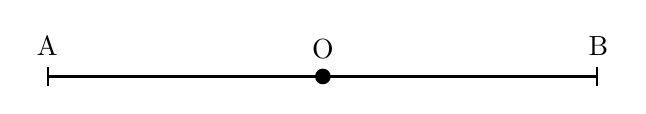
\begin{tikzpicture}[mynode/.style={fill,circle,inner sep=2pt,outer sep=0pt}
            ]
            \draw[thick] [|-|] (0,0) -- (7,0)
            node[pos=0,label=above:{A}]{}
            node[pos=0.5,mynode,label=above:{O}]{}
            node[pos=1,label=above:{B}]{};
        \end{tikzpicture}
    \end{center}
    Se tiene que\[AX+XB=AB\qquad AO=AB/2\]
    De la propiedad triangular:\begin{align*}
        AX<XB+AO\to AX<AB-AX+AB/2\to AX<\tfrac{3}{4}AB\\
        AX>XB-XO\to AX>AB-AX-AB/2\to AX>\tfrac{1}{4}AB
    \end{align*}
    Entonces tenemos que el intervalo válido para $X$ es el naranja:
    \begin{center}
        \begin{tikzpicture}
            \draw[thick] [|-|] (0,0) -- (8,0)
            node[pos=0,label=above:{A}]{}
            node[pos=0.5,label=above:{O}]{}
            node[pos=0.25,label=above:{$\tfrac{1}{4}AB$}]{}
            node[pos=0.75,label=above:{$\tfrac{3}{4}AB$}]{}
            node[pos=1,label=above:{B}]{};

            \draw[thick,orange] (2,0) -- (6,0);
            \draw[orange,thick,fill=white] (2,0) circle (0.1);
            \draw[orange,thick,fill=white] (6,0) circle (0.1);
            \draw[thick,fill=black] (4,0) circle (0.1);
        \end{tikzpicture}
    \end{center}
    \[P(\text{triángulo})=\frac{d(\tfrac{1}{4}AB,\tfrac{3}{4}AB)}{d(A,B)}=\frac{1}{2}\]